\documentclass{article}

\usepackage[final]{neurips_2019}
\usepackage[utf8]{inputenc}
\usepackage[T1]{fontenc}   
\usepackage{hyperref}      
\usepackage{url}           
\usepackage{booktabs}      
\usepackage{amsfonts}      
\usepackage{nicefrac}      
\usepackage{microtype}     
\usepackage{graphicx}
\usepackage{geometry}

\linespread{1.25}

\title{A Survey of Accessibility in Web Design}

\author{%
  Alex Agruso\\
  \texttt{aja243@txstate.edu} \\
}


\begin{document}


\begin{minipage}{0.15\textwidth}%
	
\includegraphics[width=2.0cm]{images/txst-black.jpg}
\end{minipage}%
\hfill%
\begin{minipage}{1\textwidth}\raggedright
	Department of Computer Science\\
	Texas State University\\
\end{minipage}


\maketitle


\begin{abstract}
	With the internet's current ubiquity, it is more important than ever to consider how to design accessible internet applications.
	This paper examines existing research of the accessibility of certain websites and how to design accessible websites, as well as offers critique on how to potentially improve their methods and accuracy.
\end{abstract}


\paragraph{ACM Category} Human-centered Computing > Accessibility > Accessibility design and evaluation methods
\paragraph{Keywords} Accessibility, Web Design


\section{Introduction}
In 2020, about 60\% of the global population used the internet, with that number growing to nearly 90\% in developed countries.
\cite{WorldInternetUsage}
It is easy to see that the internet has proliferated to nearly every aspect of our lives.
Applications like Canvas manage our classes, we use social media to keep in touch with others, even shopping can be done almost entirely online.
Because of this, it is important that these online applications are built to be as accessible as possible.
Otherwise, we risk compromising efficient and effective use of our applications, and in certain cases risk rendering our applications unusable by certain groups of people.

Though there are many types of applications which we could discuss, the scope of this paper will be limited to web design.
We will first exhibit evaluations of the accessibility of various websites, then discuss existing research on how to design accessible websites.
Finally, critique will be offered to improve the methods and accuracy of these studies.


\section{Website Evaluations}
A plethora of research exists assessing the accessibility of various websites.
Our paper will focus on those that analyze websites in the public sector that are likely to be used by many different types of people, including those with disabilities.


\subsection{Public Library Websites}
The first study we will examine was performed by Paul Khawaja in 2022.
\cite{Library}
In it, Khawaja seeks to assess to what extent public library websites in the United States are accessible to people with disabilities.
He did this by judging websites based on several criteria, including but not limited to compliance with various accessibility standards, e.g. WCAG and Section 508, and the existence of common accessibility issues, e.g. text on a low contrast background.

Khawaja selected a total of 120 library URLs to survey, with URLs being randomly weighted according to the population of the state the library was in to reduce selection bias.
For each URL, four key pages were tested: the website's home page, the catalog page, the events page, and the hours/location page.
An accessibility evaluation tool known as Axe was used to determine compliance with the accessibility standards.
\cite{Axe}

Using these methods, he was able to find many common accessibility flaws with the studied websites.
By far the most common type of error was color contrast errors, with them occuring nearly as much as every other type of accessibility error combined.
The other types of errors that were commonly encountered were structure errors, i.e. incorrect or inappropriate HTML tags, invalid links, poorly designed input forms, and missing alt text.
These errors were found to be common across all sites examined, as shown in figure \ref{fig:library}.

\begin{figure}
	\centering
	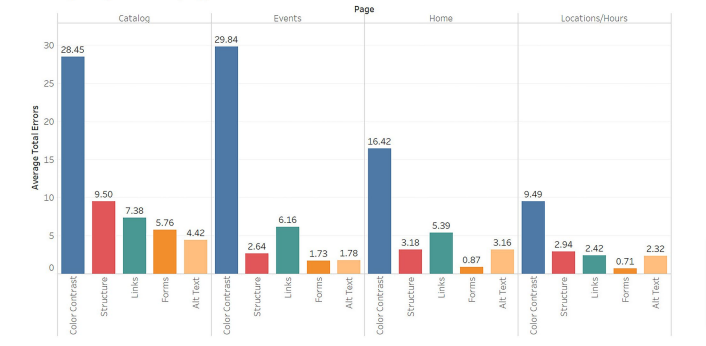
\includegraphics[width=1\textwidth]{images/librarygraph.png}
	\caption{Accessibility errors based on page category \cite{Library}}
	\label{fig:library}
\end{figure}

Khawaja also presents possible solutions to some of these errors.
For example, many browsers are capable of detecting and fixing color contrast issues dynamically, so that poor design doesn't hamper usability.
However, he also notes that some errors, especially structural errors, would require greater effort on the port of the software developer to overcome.

\subsection{Government Websites}
The next paper was published by Nishtha Kesswani and Sanjay Kumar in 2021.
\cite{Government}
In it, they perform an assessment of the accessibility of various government websites from across the globe.

They selected both developed and developing countries, specifically choosing to assess the official government websites of the G7 countries (US, Japan, UK, Germany, France, Canada, and Italy) and the BRICS countries (Brazil, Russia, India, China, and South Africa).
After compiling the data, they ultimately concluded that, while the G7 countries' websites tended to be slightly better, there was no significant correlation between a country's economic status and the accessibility of their official government website.
Rather, they found that all government websites, from both developed and developing countries, had accessibility issues, with some being dramatically worse than others.
This is illustrated in figures \ref{fig:gseven} and \ref{fig:brics}.

This lack of accessibility poses a huge problem for the people who rely on these websites, and is especially apparent in countries that do not enforce accessibility guidelines.
Ultimately, they determined that accessibility is often overlooked in the designs of government websites.

\begin{figure}
	\centering
	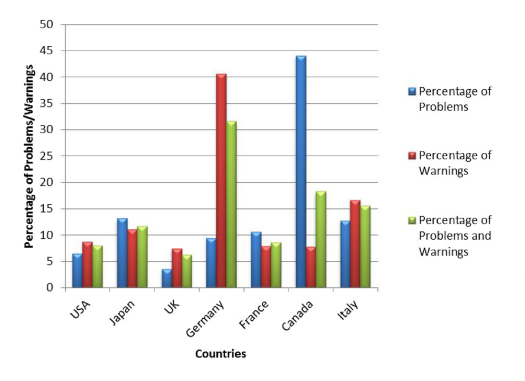
\includegraphics[width=0.6\textwidth]{images/governmentgraph1.png}
	\caption{Accessibility warnings of G7 countries \cite{Government}}
	\label{fig:gseven}
\end{figure}

\begin{figure}
	\centering
	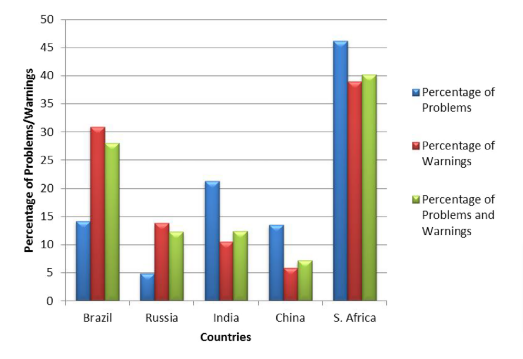
\includegraphics[width=0.6\textwidth]{images/governmentgraph2.png}
	\caption{Accessibility warnings of BRICS countries \cite{Government}}
	\label{fig:brics}
\end{figure}

\subsection{Educational Websites}
Finally, we 


\section{How to Design Accessible Websites}
Now that we understand the importance of accessibility in web design, we can now look at methods of ensuring accessibility in the websites we build.

\subsection{How to Teach Accessible Design}
In 2020, Michael Whitney published a paper on integrating accessibility principles into web design courses.
He discusses the importance of teaching accessibility in web design, and how most modern web design treats accessibility with little importance.
\cite{Learning}

In his paper, Whitney emphasizes the importance of teaching how to properly assess a website's accessibility.
Specifically, he proposes teaching specific accessibility guidelines such as the Web Content Accessibility Guidelines (WCAG), created by the W3C in an effort to proliferate web accessibility.
The WCAG specifies three different levels of conformance: A, AA, and AAA, with each level being stricter than the last.
When web designers have a clear criteria for judging accessibility, they have a clear image of what must be done in order to make the website accessible.

Whitney also discusses the importance of using accessibility assessment tools.
Specificy, he talks about W3C's Markup Validation Service, which provides detailed issues about a website, including those related to accessibility.
This tool automates a lot of the validation work that goes in to ensuring accessibility, and thus better enables developers to implement accessible designs.

Finally, Whitney talks about the challenges that teachers face when integrating accessibility into their teaching.
He notes a lacking in many faculty's accessibility expertise, which naturally leads to a lacking of accessibility in their curriculum.
He also noted that students tended not to program according to accessibility guidelines unless explicity required to do so.
Consequently, he advocates for a consistent and strict requirement of accessibility in student's work in order to establish a habit of thinking about accessible designs.


\section{Critical Assessment}
Overall, I feel that all of the studies discussed in this paper do a good job in bringing certain accessibility issues to light.
Khawaja's paper in particular shows that color constrast design flaws are the most common type of accessibility error, but also the easiest to fix.
Consistently applying this knowledge when designing websites would eliminate a large class of accessibility errors and make websites more accessible to individuals with visual impairment.
Additionally, Kesswani and Kumar's paper highlights the issues that exist with the accessibility of government websites, as well as the conseqeunces of this lack of accessibility.

On aspect in which these papers could have improved would be their scope.
I feel as if their sample sizes were fairly limited, especially Kesswani and Kumar's paper.
They could have chosen so


\section{Future Work}
Now that we know some areas of the internet which lack accessiblity, we can try to think of ways of filling these accessibility gaps.
Potential solutions could include a browser plugin that dynamically converts website code into a form that is more accessible to the user.
However, such a program would be difficult to generalize to all cases, as website design can be incredibly varied.
This could also present as an opportunity to put AI to work.
We could train an AI model on accessible web designs and have it judge or modify human made websites according to its training.
AI capabilities are still rapidly improving, so it is not out of the realm of possibility that something like this could happen, but it would likely require a large commitment of effort to achieve something that is usefu.


\section{Conclusion}
Clearly, accessibility is incredibly important in web design.
Not only does it allow equal access to web resources for those who are disabled, but it allows even non-disabled users to more effectly use the websites that they visit.

It is also apparent that many important websites lack accessibility features.


\small
\bibliographystyle{plain}
\bibliography{references}


\end{document}

